% Experimental Evaluation
\section{Experimental Evaluation}

    \subsection{First Steps}
        As a natural continuation of the methodological design, the experimental evaluation began with a deliberately simplified implementation. Our intention at this stage was not to prove the final effectiveness of the system, but rather to verify that the pipeline---from simulation environment to training and logging, and finally to analysis and visualization---was functioning in practice. To do this, we chose to start with a two-dimensional environment. This decision was motivated by two main reasons: on the one hand, it drastically reduces computational and implementation complexity compared to a full 3D quadrotor simulation; on the other hand, it allows much faster iteration cycles, enabling us to quickly observe whether the learning dynamics of the swarm produced any coherent behavior or if everything remained random noise. In other words, the 2D environment represented the most direct way to put the theoretical framework to the test and obtain immediate feedback.
        \medskip

    \subsection{Setup (Common Across P0--P1)}
        We consider a planar interception task in discrete time $t=0,1,\dots$, where a drone agent must reach a fixed target. The agent observes a normalized state vector
        \begin{equation}
            \label{eq:obs}
            \mathbf{o}_t \;=\; \frac{1}{\max(1,\,\texttt{plane}-1)}\,[\,x_t,\,y_t,\,x^{(\mathrm{tar})},\,y^{(\mathrm{tar})}\,] \in [0,1]^4,
        \end{equation}
        with $(x_t,y_t)$ the drone cell and $(x^{(\mathrm{tar})},y^{(\mathrm{tar})})$ the target cell.\footnote{Normalization as implemented in \texttt{\_norm\_obs}, denominator $\max(1,\texttt{plane}-1)$.}
        \medskip

        At each step, the agent selects a discrete action $a_t\in\mathcal{A}$ that moves the drone by a displacement $(\Delta x,\Delta y)$ clipped within the arena bounds; next state, Euclidean distance $d_t$, and termination are computed accordingly.\footnote{Environment step: integer grid move, clamped to $[0,\texttt{plane}-1]$, with termination on $d_t\le\varepsilon$ or $t\ge\texttt{MAX\_STEPS}$.}

        \subsubsection{Reward shaping.}
            Let $d_t$ be the Euclidean drone–target distance and $d_{\max}=\sqrt{2}\,(\texttt{plane}-1)$ the maximum diagonal distance. The per-step reward is
            \begin{align}
                r_t \;=\; &\underbrace{K \big(\tfrac{d_{t-1}}{d_{\max}}-\tfrac{d_t}{d_{\max}}\big)}_{\text{progress (normalized)}} \;-\; \underbrace{c_{\mathrm{step}}}_{\text{step cost}}
                \;-\; \underbrace{c_{\mathrm{turn}}\,[a_t\neq a_{t-1}]}_{\text{turn penalty}}
                \;-\; \underbrace{c_{\mathrm{rev}}\,[s_t\in\mathcal{V}]}_{\text{revisit penalty}}, \label{eq:reward}\\
                &\text{plus terminal terms:}\quad
                \begin{cases}
                +R\,(1+\tfrac{T_{\max}-t}{T_{\max}}) & \text{if } d_t\le \varepsilon \\
                - R_{\mathrm{to}} & \text{if } t\!=\!T_{\max}
                \end{cases}\nonumber
            \end{align}
            with $K=1.0$, $c_{\mathrm{step}}{=}0.003$, $c_{\mathrm{turn}}{=}0.002$, $c_{\mathrm{rev}}{=}0.01$, $R{=}20.0$, $R_{\mathrm{to}}{=}1.0$ in the large-grid setting; the success threshold is $\varepsilon=\max(1.0,0.005\cdot \texttt{PLANE\_SIZE})$.%

            This is a potential-based shaping on $d_t$ (distance) plus small control-like regularizers.

        \subsubsection{Learning.}
            In P0--P1 we use a neural $Q$-function $Q_\theta(\mathbf{o},a)$ trained with Double DQN and a target network. The function approximator is a 2-layer MLP (256–256 ReLU) with $|\mathcal{A}|$ outputs, Huber loss, gradient clipping, and Adam optimizer.\footnote{Architecture and update: 2-layer MLP (256,256) → $|\mathcal{A}|$; Double DQN target with online $\arg\max$ and target gather; Huber loss; grad clip at 5.0; Adam with $\mathrm{lr}=1.5\mathrm{e}{-3}$.}
            Exploration is $\varepsilon$-greedy with linear decay $\varepsilon(s)$ from $0.25$ to $0.02$ over $150\text{k}$ steps; replay buffer size $3\!\times\!10^5$, batch $256$, $\gamma=0.99$, target sync every $2\text{k}$ updates.

        \subsubsection{Evaluation.}
            We report success rate ($\%$ of episodes reaching $d_t\le\varepsilon$), average return (shaped), and average steps, via a greedy policy ($\arg\max_a Q$) on uniformly random spawns over the full arena. For visualization, we use an offline \emph{play} that reproduces the same observation normalization and arena parameters (\texttt{plane}, \texttt{MAX\_STEPS}, $\varepsilon$) saved in the training checkpoint.\footnote{The playback environment uses identical normalization (Eq.~\eqref{eq:obs}) and termination to avoid train–eval mismatch.}

    \subsection{P0 — Tiny Grid (small 2D grid, 4 directions + stay)}
        \subsubsection{Objective.}
            Sanity-check the full pipeline (environment, reward shaping, logging, evaluation) and verify that the learned policy develops a consistent homing behavior on a small grid with $|\mathcal{A}|=5$ (N/S/E/W + stay).

        \subsubsection{Methodology.}
            Same $Q_\theta$ architecture (smaller action set). Reward shaping as in Eq.~\eqref{eq:reward} with the same structure; smaller arena implies a larger per-step progress signal $\Delta d/d_{\max}$ and naturally easier credit assignment.

        \subsubsection{Results.}
            Across seeds, training curves show a monotonic rise in success with diminishing variance; representative windows reached $\approx 70\%\!\to\!90\%$ success as training proceeds (consistent with step-wise shaped returns improving over time). Qualitative rollouts show direct, low-zigzag homing; near-target corrections are mild due to the small $c_{\mathrm{turn}}$ and the positive progress term.

        \subsubsection{Takeaways.}
            The shaping in Eq.~\eqref{eq:reward} is sufficient to break symmetry and converge quickly on small grids; the observation normalization in Eq.~\eqref{eq:obs} prevents scale issues and enables reuse on larger arenas.

    \subsection{P1 — Big Grid DQN (101$\times$101, 8 directions + stay)}
        \subsubsection{Objective.}
            Scale to a larger arena (\texttt{PLANE\_SIZE}$=101$), expand the action set to 8 compass moves + stay ($|\mathcal{A}|=9$), and validate stability of Double DQN under sparse terminal rewards.

        \subsubsection{Curriculum on spawn distance.}
            To unlock early successes and propagate terminal value, we constrain the initial Manhattan distance $\|p_0 - p_0^{(\mathrm{tar})}\|_1 \le D_{\max}(e)$ with a schedule
            \[
            D_{\max}(e)=
            \begin{cases}
            20,& e<500\\
            40,& 500\le e<2000\\
            \texttt{PLANE\_SIZE},& e\ge 2000
            \end{cases}
            \]
            where $e$ is the episode index; beyond $e\!\ge\!2000$ we use full-arena spawns.\footnote{Spawn curriculum implemented in \texttt{reset(episode)} with \texttt{max\_spawn\_manhattan\_for\_episode}.}

        \subsubsection{Reward calibration.}
            On a $101\times 101$ grid the unit progress is $\Delta d/d_{\max}\approx 1/\sqrt{2}\,(\texttt{plane}-1)^{-1}\approx 0.007$, hence we lower $c_{\mathrm{turn}}$ to $0.002$ and $c_{\mathrm{step}}$ to $0.003$ so that a single correct move near the target remains net-positive; the arrival bonus $R{=}20$ ensures rare successes dominate return and backpropagate through bootstrapping.\footnote{Large-grid constants used: $c_{\mathrm{turn}}{=}0.002$, $c_{\mathrm{step}}{=}0.003$, $R{=}20$.}

        \subsubsection{Training configuration.}
            We train for up to $1000$ episodes with replay $3\!\times\!10^5$, batch 256, $\gamma=0.99$, Adam ($1.5\!\times\!10^{-3}$), target sync every $2000$ updates, $\varepsilon$-greedy from $0.25$ to $0.02$ over $150$k steps, gradient clip $5.0$.
            The observation normalization, termination, and evaluation are identical to training to avoid distribution shift.

        \subsubsection{Metrics and representative outcome.}
            We monitor success rate, shaped average return, and average steps. In a representative large-grid run, the training summary reported
            \emph{[Ep 1000] avg\_return = 39.116, $\varepsilon=0.101$, success\_rate = 87.80\%}.%
            % (User-provided log)
            Qualitatively, evaluation rollouts (pure $\arg\max$) reach the target without orbiting; the reduction of $c_{\mathrm{turn}}$ removes pathological near-target zigzag and improves closure.

            \begin{figure}[H]
                \centering
                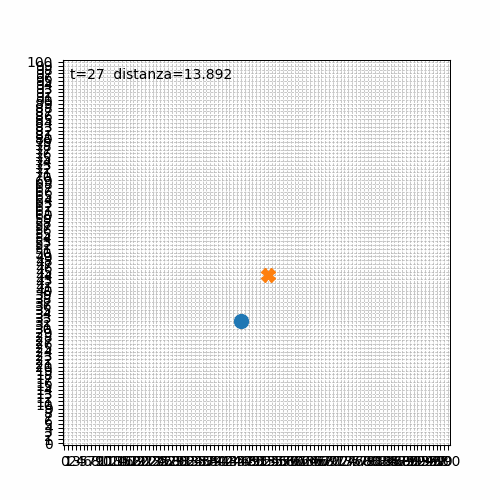
\includegraphics[scale=0.5]{Figures/step_2_t2.png}
                \caption{Representative greedy rollout on the large grid (P1). The agent closes on the target with minimal zigzag. Animated version can be found on our \underline{\href{https://github.com/rolandoinnamorati/swarm-rl}{GitHub repository.}}}
            \end{figure}
